% Document class and imports
\documentclass[english, aspectratio=169]{beamer}
\usepackage[utf8]{inputenc}
\usepackage[TS1,T1]{fontenc}
\usepackage{babel}
\usepackage{bm}% bold math
\usepackage{mathtools}
\usepackage{subfig}
\usepackage{tabularx}
\usepackage{booktabs}
% metadata
\usetheme{CASUS}
\title[MALA background]{MALA background} 
\subtitle{Part of the tutorial on MALA}
\author{Lenz Fiedler}
\date{21.03.2022}

% Commands
\newcommand{\br}{\bm{r}}
\newcommand{\bR}{\bm{R}}
\newcommand{\ubr}{\underline{\bm{r}}}
\newcommand{\ubR}{\underline{\bm{R}}}
\newcommand{\bu}{{\bf u}}
\newcommand{\bU}{{\bf U}}
\newcommand{\bF}{{\bf F}}
\newcommand{\s}{_\mathrm{{\scriptscriptstyle S}}}
\newcommand{\h}{_\mathrm{{\scriptscriptstyle H}}}
\newcommand{\xc}{_\mathrm{{\scriptscriptstyle XC}}}
\newcommand{\hxc}{_\mathrm{{\scriptscriptstyle HXC}}}
\newcommand{\bk}{\bm{k}}
\newcommand{\Kelvin}{\mathrm{K}}
\newcommand{\zerotemp}{^{\scriptscriptstyle T=0\mathrm{K}}}
\newcommand{\nonzerotemp}{^{\scriptscriptstyle T>0\mathrm{K}}}
\newcommand{\kB}{k_\mathrm{B}}

\definecolor{cred}{RGB}{150,38,76}
\definecolor{cblue}{RGB}{0,80,150}
\definecolor{cgreen}{RGB}{160,227,0}
\definecolor{corange}{RGB}{255,166,0}
\newcommand{\yellow}[1]{\noindent{{\color{yellow!60!black} #1}}}
\newcommand{\green}[1]{\noindent{{\color{green!60!black} #1}}}
\newcommand{\blue}[1]{\noindent{{\color{blue!60!black}  #1}}}

\begin{document}
	\titleframe
	\contentsframe
	\section{ }
	\begin{frame}{MALA workflow}
		\centering
		\vspace{-0.5cm}
		\visible<1>{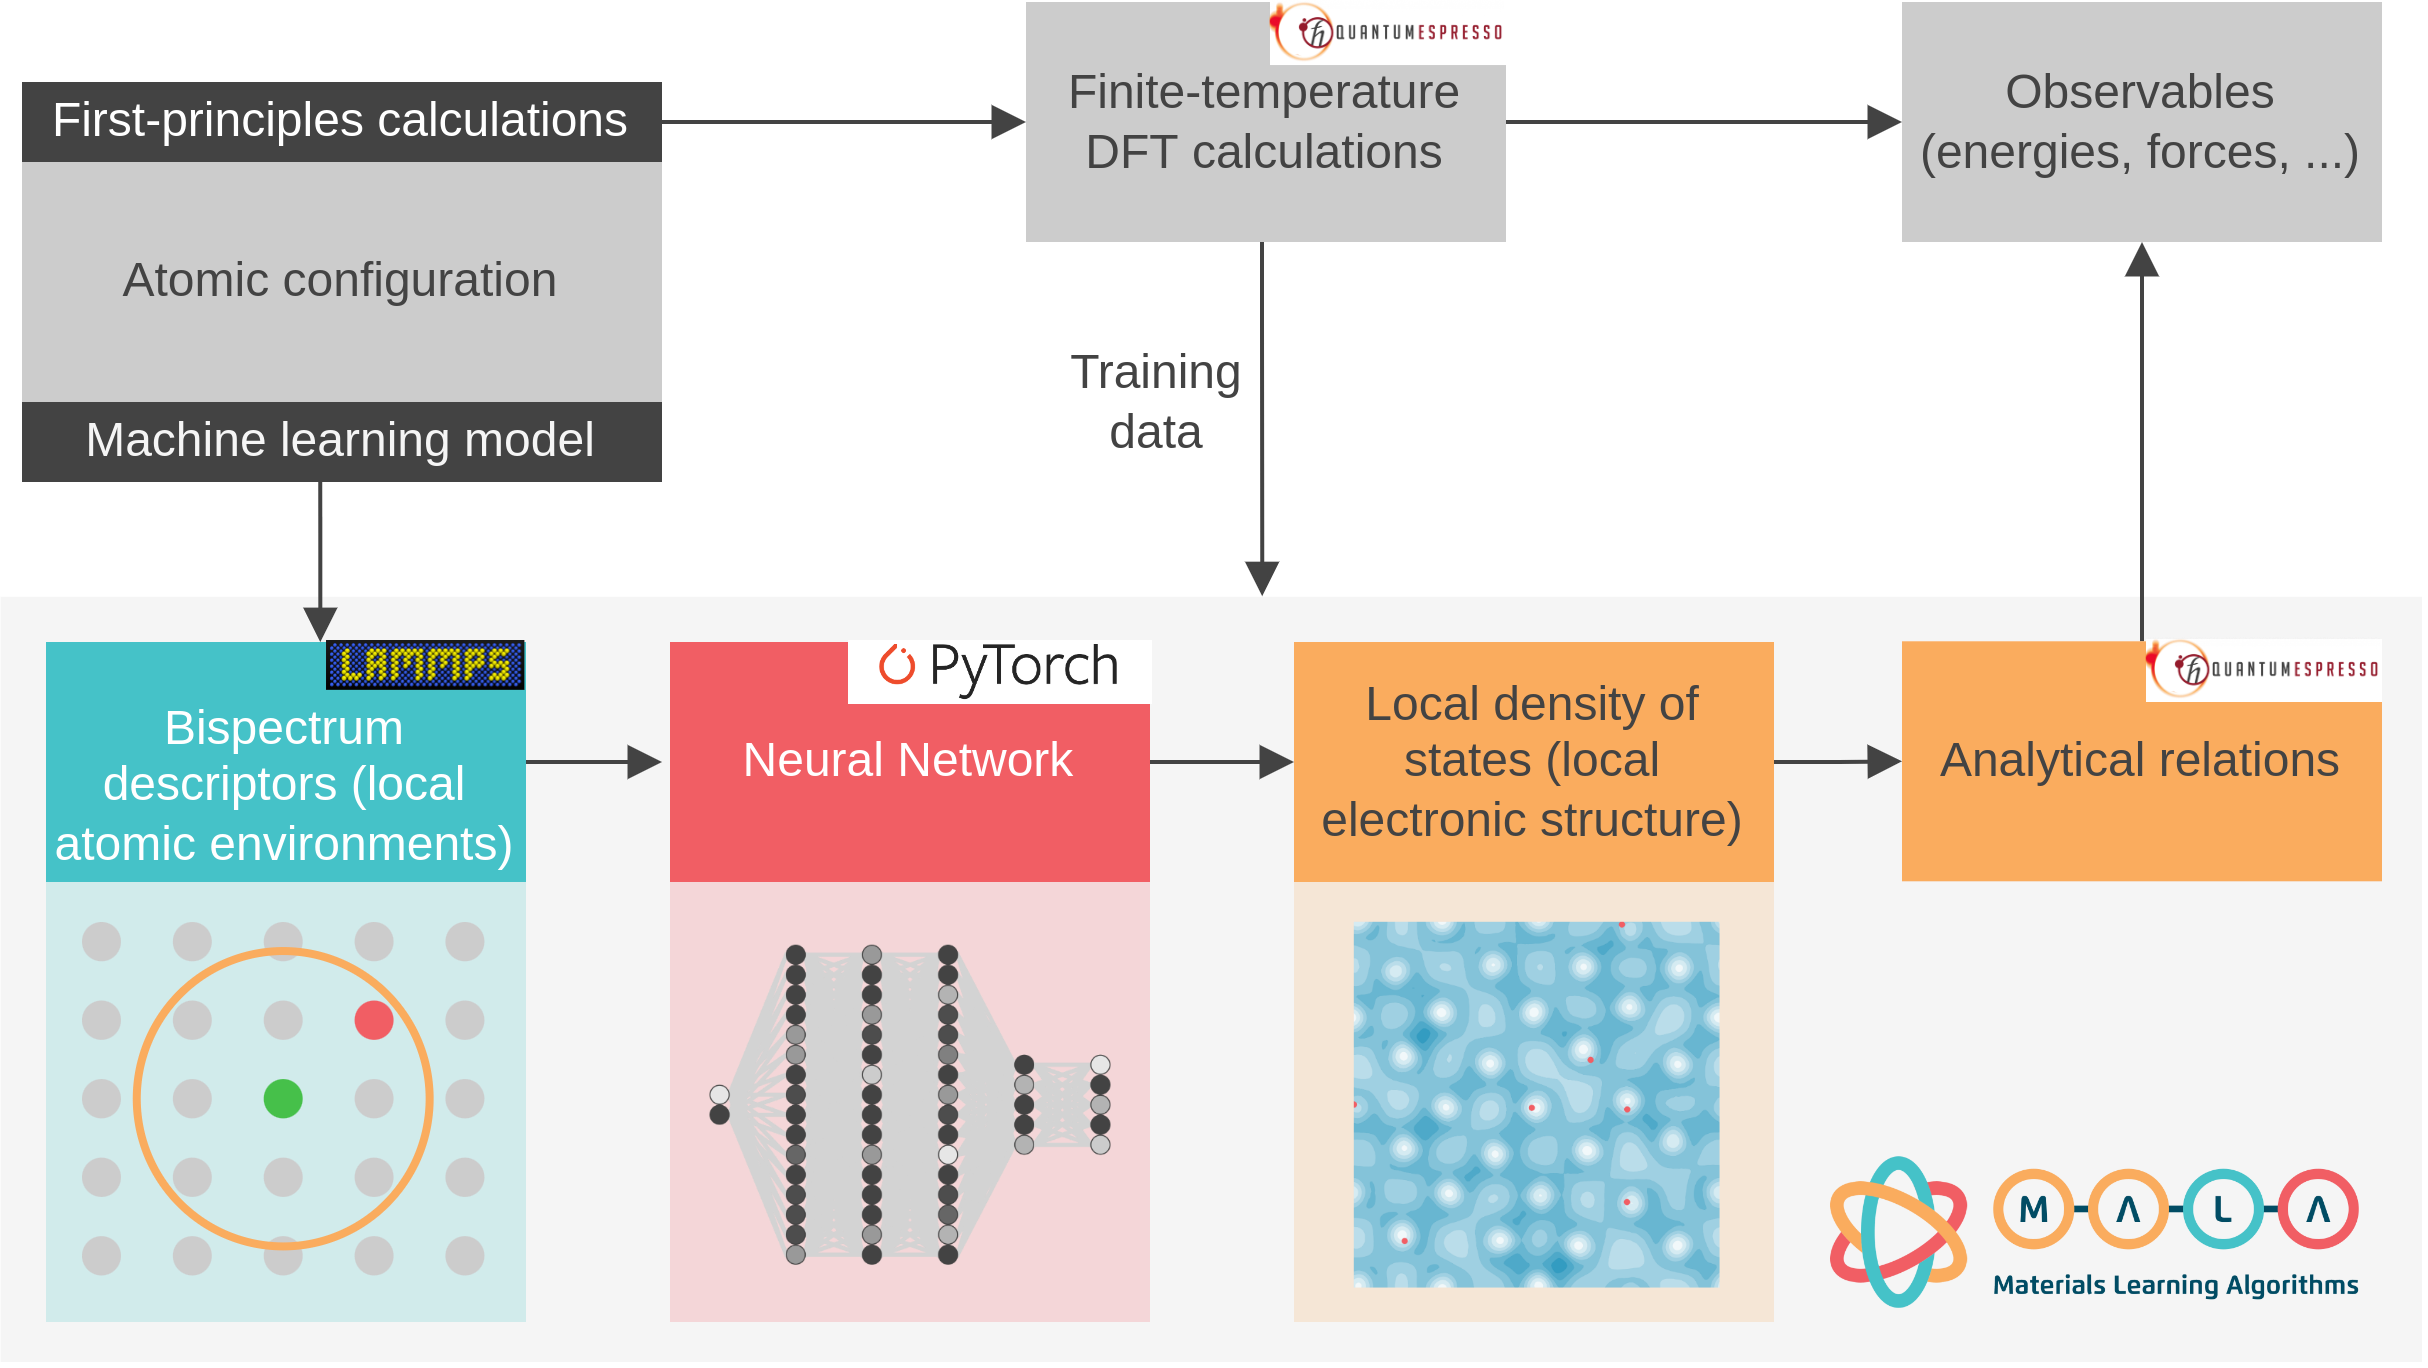
\includegraphics[width=0.75\textwidth]{figures/mala_workflow.png}}
	\end{frame}
	\begin{frame}{Relevant equations}
	\begin{align}
		\visible<1->{\tilde{d}(\epsilon, \br) = &M(B(\,J, \br)) \nonumber \\}
		\visible<2->{n(\br) = & \int d \epsilon\;  f^\tau(\epsilon) d(\epsilon, \br) \; \nonumber \\
	        D(\epsilon) =  &\int d\br \; d(\epsilon, \br)  \nonumber \\}
		\visible<3->{A[n] = A[n[d], D[d]] = &E_b[D[d]]-\kB\tau S_\mathrm{S}[D[d]]-E_\mathrm{H}[n[d]] \nonumber \\ \nonumber &+E_\mathrm{XC}-\int d \br v_\mathrm{XC}(\br)n[d](\br)+E_{ii}}
	\end{align}
	\end{frame}
	\begin{frame}{MALA publications}
		\centering
		\vspace{0pt}
		\begin{itemize}\setlength\itemsep{0.5em}
			\item Accelerating finite-temperature Kohn-Sham density functional theory with deep neural networks, J. A. Ellis, \textit{et al} 2021 \textit{Phys. Rev. B 104}, 035120  \pause
			\item Training-free hyperparameter optimization of neural networks for electronic structures in matter, L. Fiedler \textit{et al} 2022 \textit{Mach. Learn.: Sci. Technol.} \textbf{3} 045008 \pause 
			\item Predicting electronic structures at any length scale with machine learning, L. Fiedler \textit{et al}, publication pending, \textit{arXiv:2210.11343} \pause
			\item Check MALA out on GitHub: https://github.com/mala-project
		\end{itemize}
	\end{frame}
	\begin{frame}{MALA cooperation partners}
		\centering
		\vspace{0pt}
		
\includegraphics[width=0.4\linewidth]{figures/sandia}
		
\includegraphics[width=0.4\linewidth]{figures/ornl}
		
\includegraphics[width=0.45\linewidth]{figures/casus} \\
	\end{frame}
	\presentationendframe
%	\begin{frame}{Dwarfs as seen from microbes}
%		\dots provide lots of good places for embarkation.
%	\end{frame}


\end{document}
